\documentclass{article}

\usepackage{epsfig}
\usepackage[mathscr]{eucal}
\usepackage{amsfonts}
\usepackage{amscd}
\usepackage{amsmath}
\usepackage{array}
\usepackage{amssymb}
%\usepackage[backend=bibtex8, sorting=none]{biblatex}
\usepackage{colordvi}
\usepackage{enumerate}
\usepackage{graphicx}
\usepackage{booktabs}
\usepackage[footnotesize]{caption}
\usepackage{fancyhdr}
\usepackage{pdfpages}
\usepackage{slashed}
\usepackage{tabularx}
\usepackage{longtable}
\usepackage{array}
\usepackage{caption}
\usepackage{subcaption}

%\usepackage{relsize}
\usepackage{color}
\usepackage{rotating}

\usepackage{slashed}

\usepackage{epsfig,amsmath,graphicx,amssymb,listings,slashed}
\usepackage[colorlinks,citecolor=blue,urlcolor=blue,linkcolor=blue]{hyperref}
\usepackage[outercaption]{sidecap}

\usepackage{booktabs}

%\smartqed
%\usepackage[T1]{fontenc}
\usepackage[utf8]{inputenc}

\usepackage{epsfig,amsmath,graphicx,amssymb,listings,slashed}
\usepackage[colorlinks,citecolor=blue,urlcolor=blue,linkcolor=blue]{hyperref}

\setlength{\evensidemargin}{0cm}
\setlength{\oddsidemargin}{0cm}
\setlength{\topmargin}{0.00cm}
\setlength{\textwidth}{16.0cm}
\setlength{\textheight}{24.00cm}
\setlength{\headheight}{0cm}
\setlength{\headsep}{0cm}
\setlength{\voffset}{0cm}
\setlength{\paperheight}{29cm}

\definecolor{ourbrown}{RGB}{155,100,15}
\definecolor{ourcyan}{RGB}{20,165,165}
\definecolor{ourpurple}{RGB}{145,0,140}
\definecolor{darkorange}{RGB}{225,100,0}
\definecolor{darkgreen}{RGB}{0,170,0}
\definecolor{darkgray}{RGB}{80,80,80}

\setlength{\marginparwidth}{20mm}







\begin{document}

\title{ Machine Learning - SS 2021 \\ Exercise 3: Synthetic Data }


	\author{Federico Ambrogi, \textcolor{blue} {e1449911@student.tuwien.ac.at } \\
	Adam Höfler, \textcolor{blue} {e11847620@student.tuwien.ac.at } \\
	Matteo Panzeri \textcolor{blue}{12039996@student.tuwien.ac.at } \\
    TU Wien }


%\ead{federico.ambrogi@univie.ac.at}




\maketitle
\setcounter{tocdepth}{2}
\tableofcontents

\section*{Introduction}
In this document we describe the results of the implementation of synthesizing algorithms to create synthetic replicas of three different data sets. We test them for their ability to create replicas of the original data set.



\section{Data Sets Description}
Here we briefly introduce our datasets, analyze the distributions of the input data and check for significant correlations between variables.


\subsection{Income Data Set}
The distribution of the relevant features, as well as a scatter plot to highlight pair-wise correlations are shown in Fig. \ref{pairplot_income}, while a more general view on the correlations are shown in Fig. \ref{correlation_income}.\\
The data set \cite{income} provides us information about people, like: age, workclass, education, marital-status, occupation, capital-gain, ecc...\\
Our purpose is to determine if a person income is lower or greater than a given value specifically the threshold is 50000 Dollars per year.

\begin{figure}[h!]
	\centering
	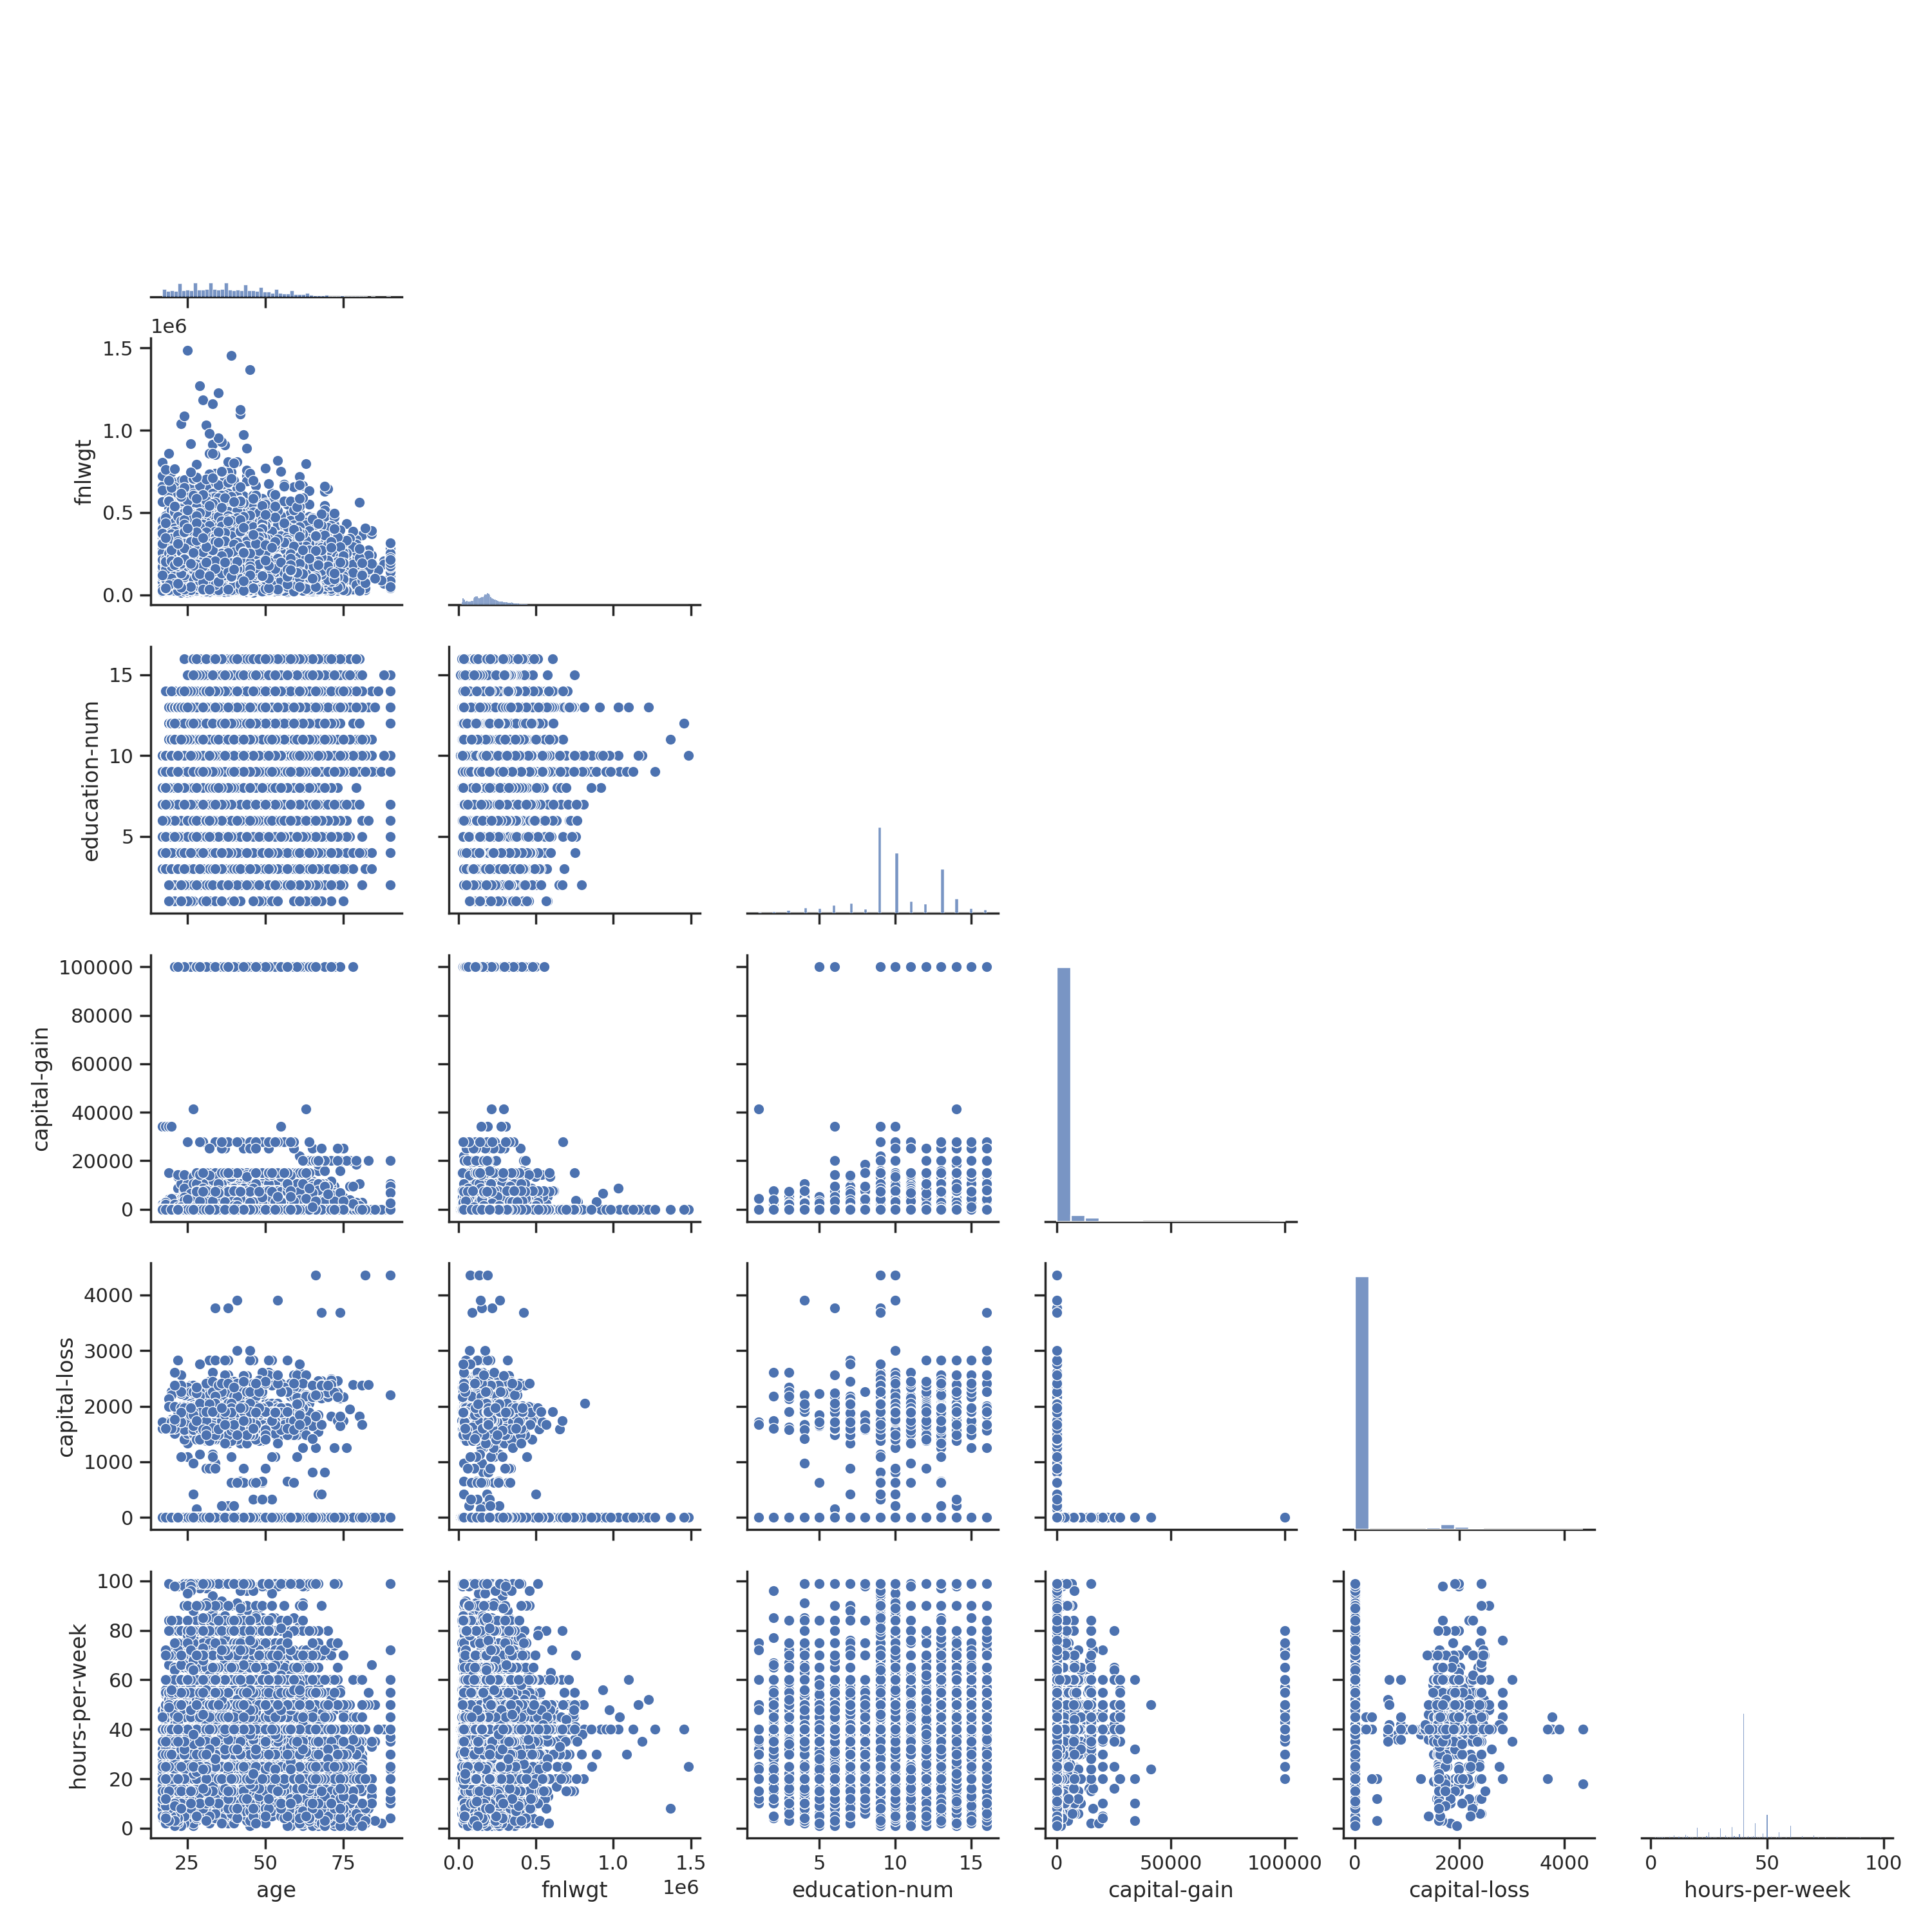
\includegraphics[width=\textwidth]{../plots/income_pairplot.png}
	\caption{ Distributions and pair-wise correlation for the features of the "income" data set.}
	\label{pairplot_income}
\end{figure}


\begin{figure}[h!]
	\centering
	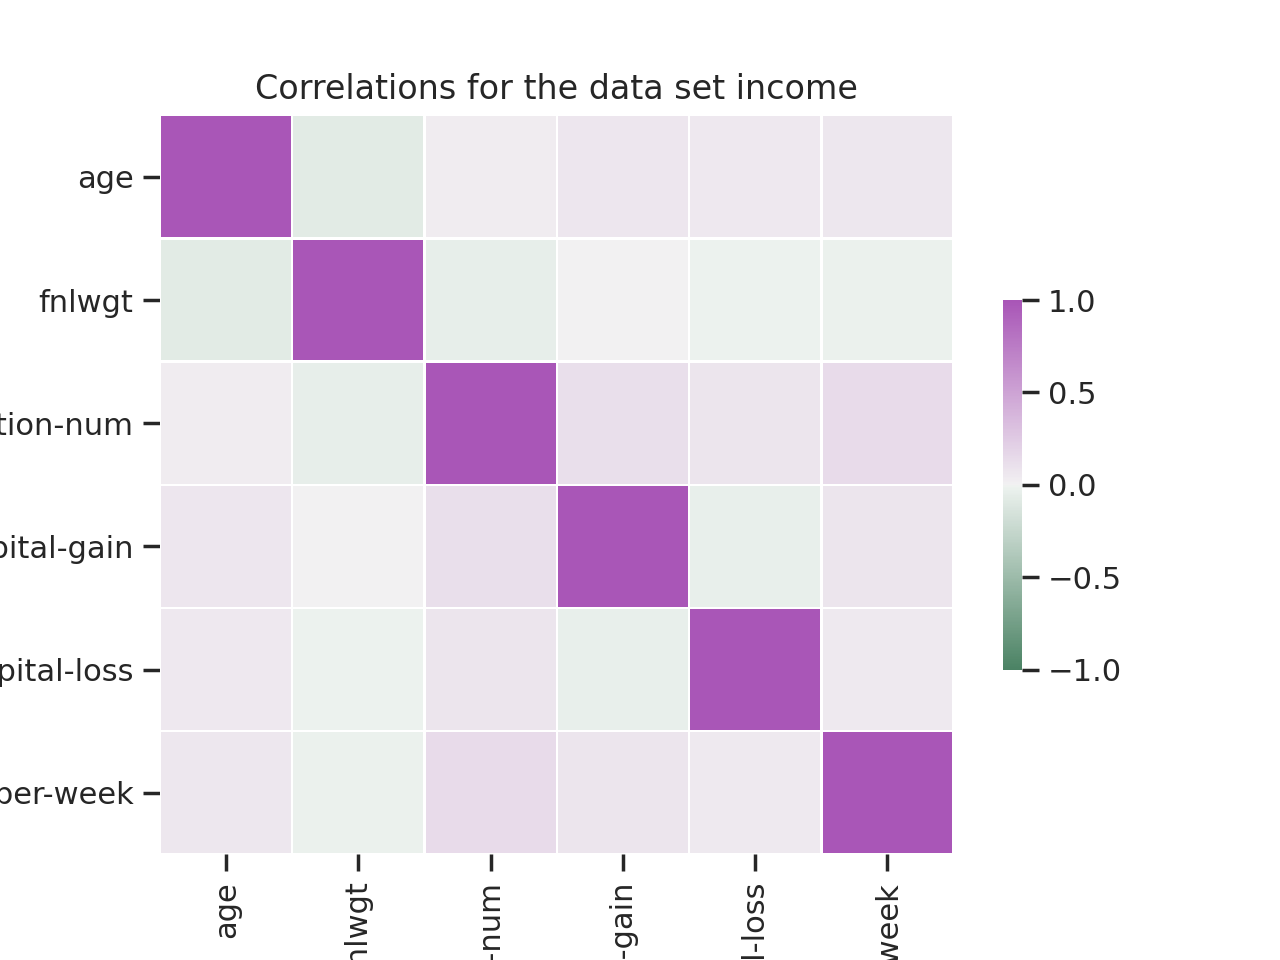
\includegraphics[width=0.7\textwidth]{../plots/income_correlations.png}
	\caption{Correlation matrix for the "income" data set. }
	\label{correlation_income}
\end{figure}



\subsection{Titanic Data Set}
The Titanic data set \cite{titanic} contains informations about the Titanic's passengers. Given the observations we want to determine if a given person, represented by an observation, will survive on the Titanic.\\
Some features of the dataset are: Name, sex, age, Passenger class, ticket fare, where the passenger embarked, etc.

\begin{figure}[h!]
	\centering
	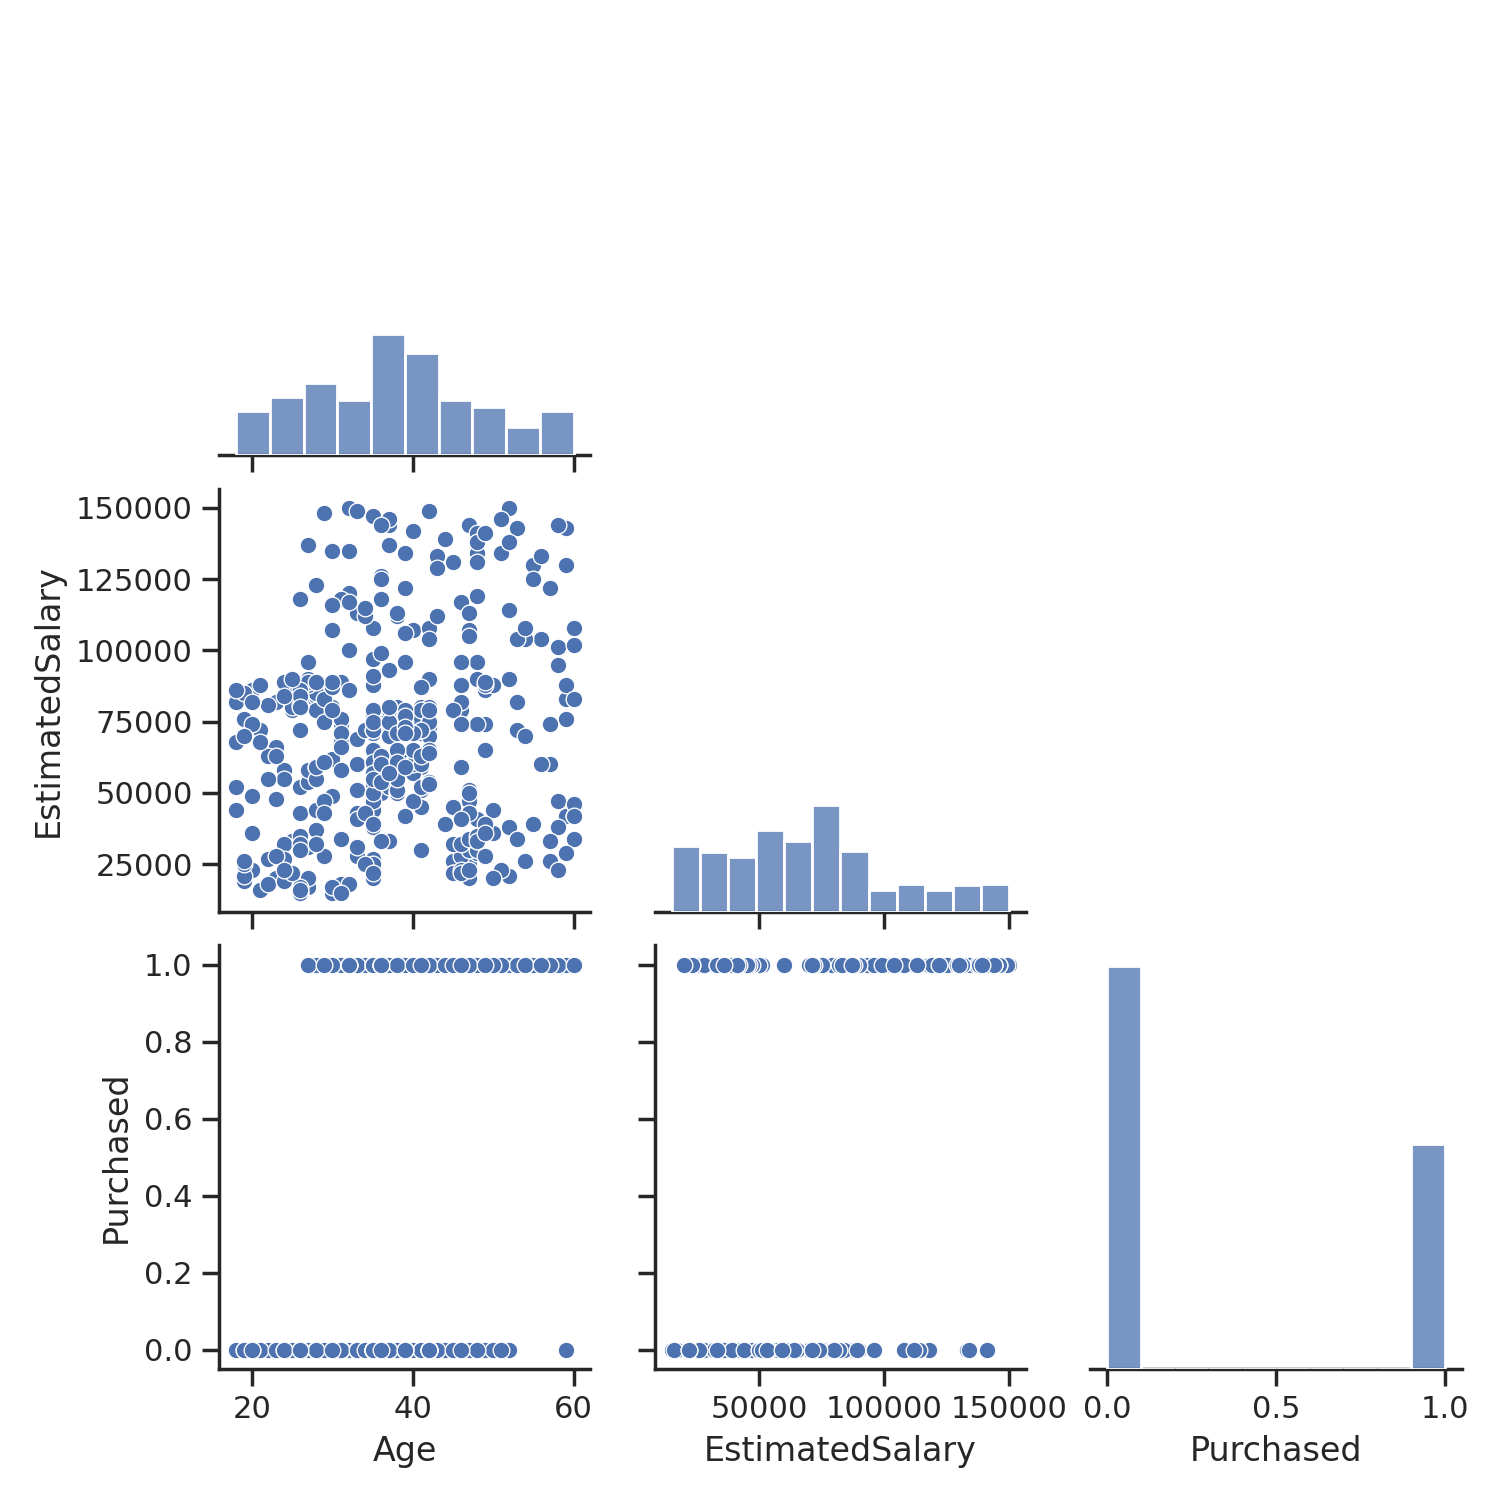
\includegraphics[width=\textwidth]{../plots/social_pairplot.png}
	\caption{ Distributions and pair-wise correlation for the features of the "social" data set.}
	\label{pairplot_income}
\end{figure}


\begin{figure}[h!]
	\centering
	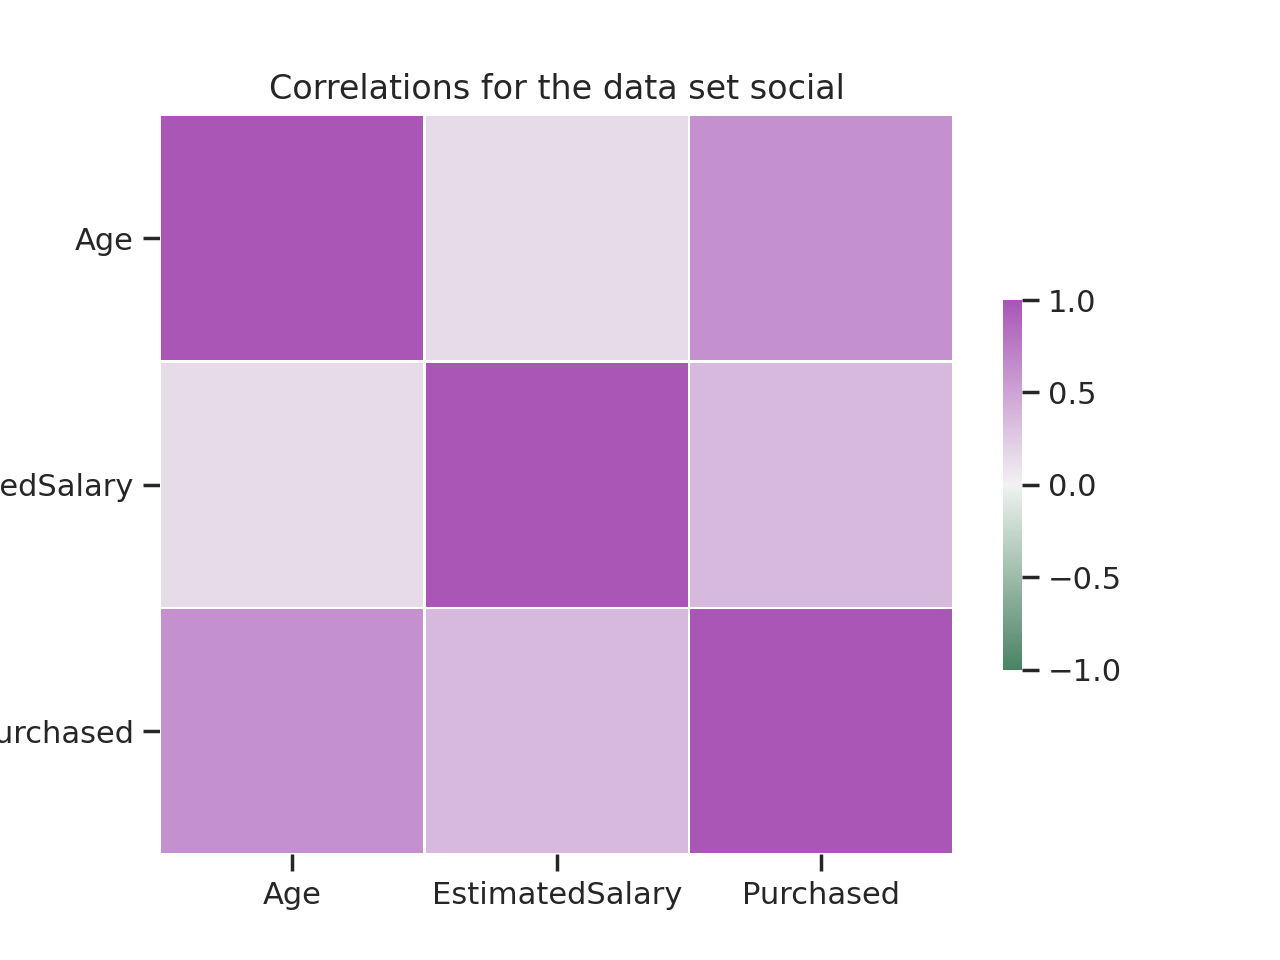
\includegraphics[width=0.7\textwidth]{../plots/social_correlations.png}
	\caption{Correlation matrix for the "social" data set. }
	\label{correlation_income}
\end{figure}



\subsection{Social Data Set}
The Social network ads data set \cite{social} collects information about social network users in particular age,sex and income. Our objective is to understand if an user will buy the advised good.

\begin{figure}[h!]
	\centering
	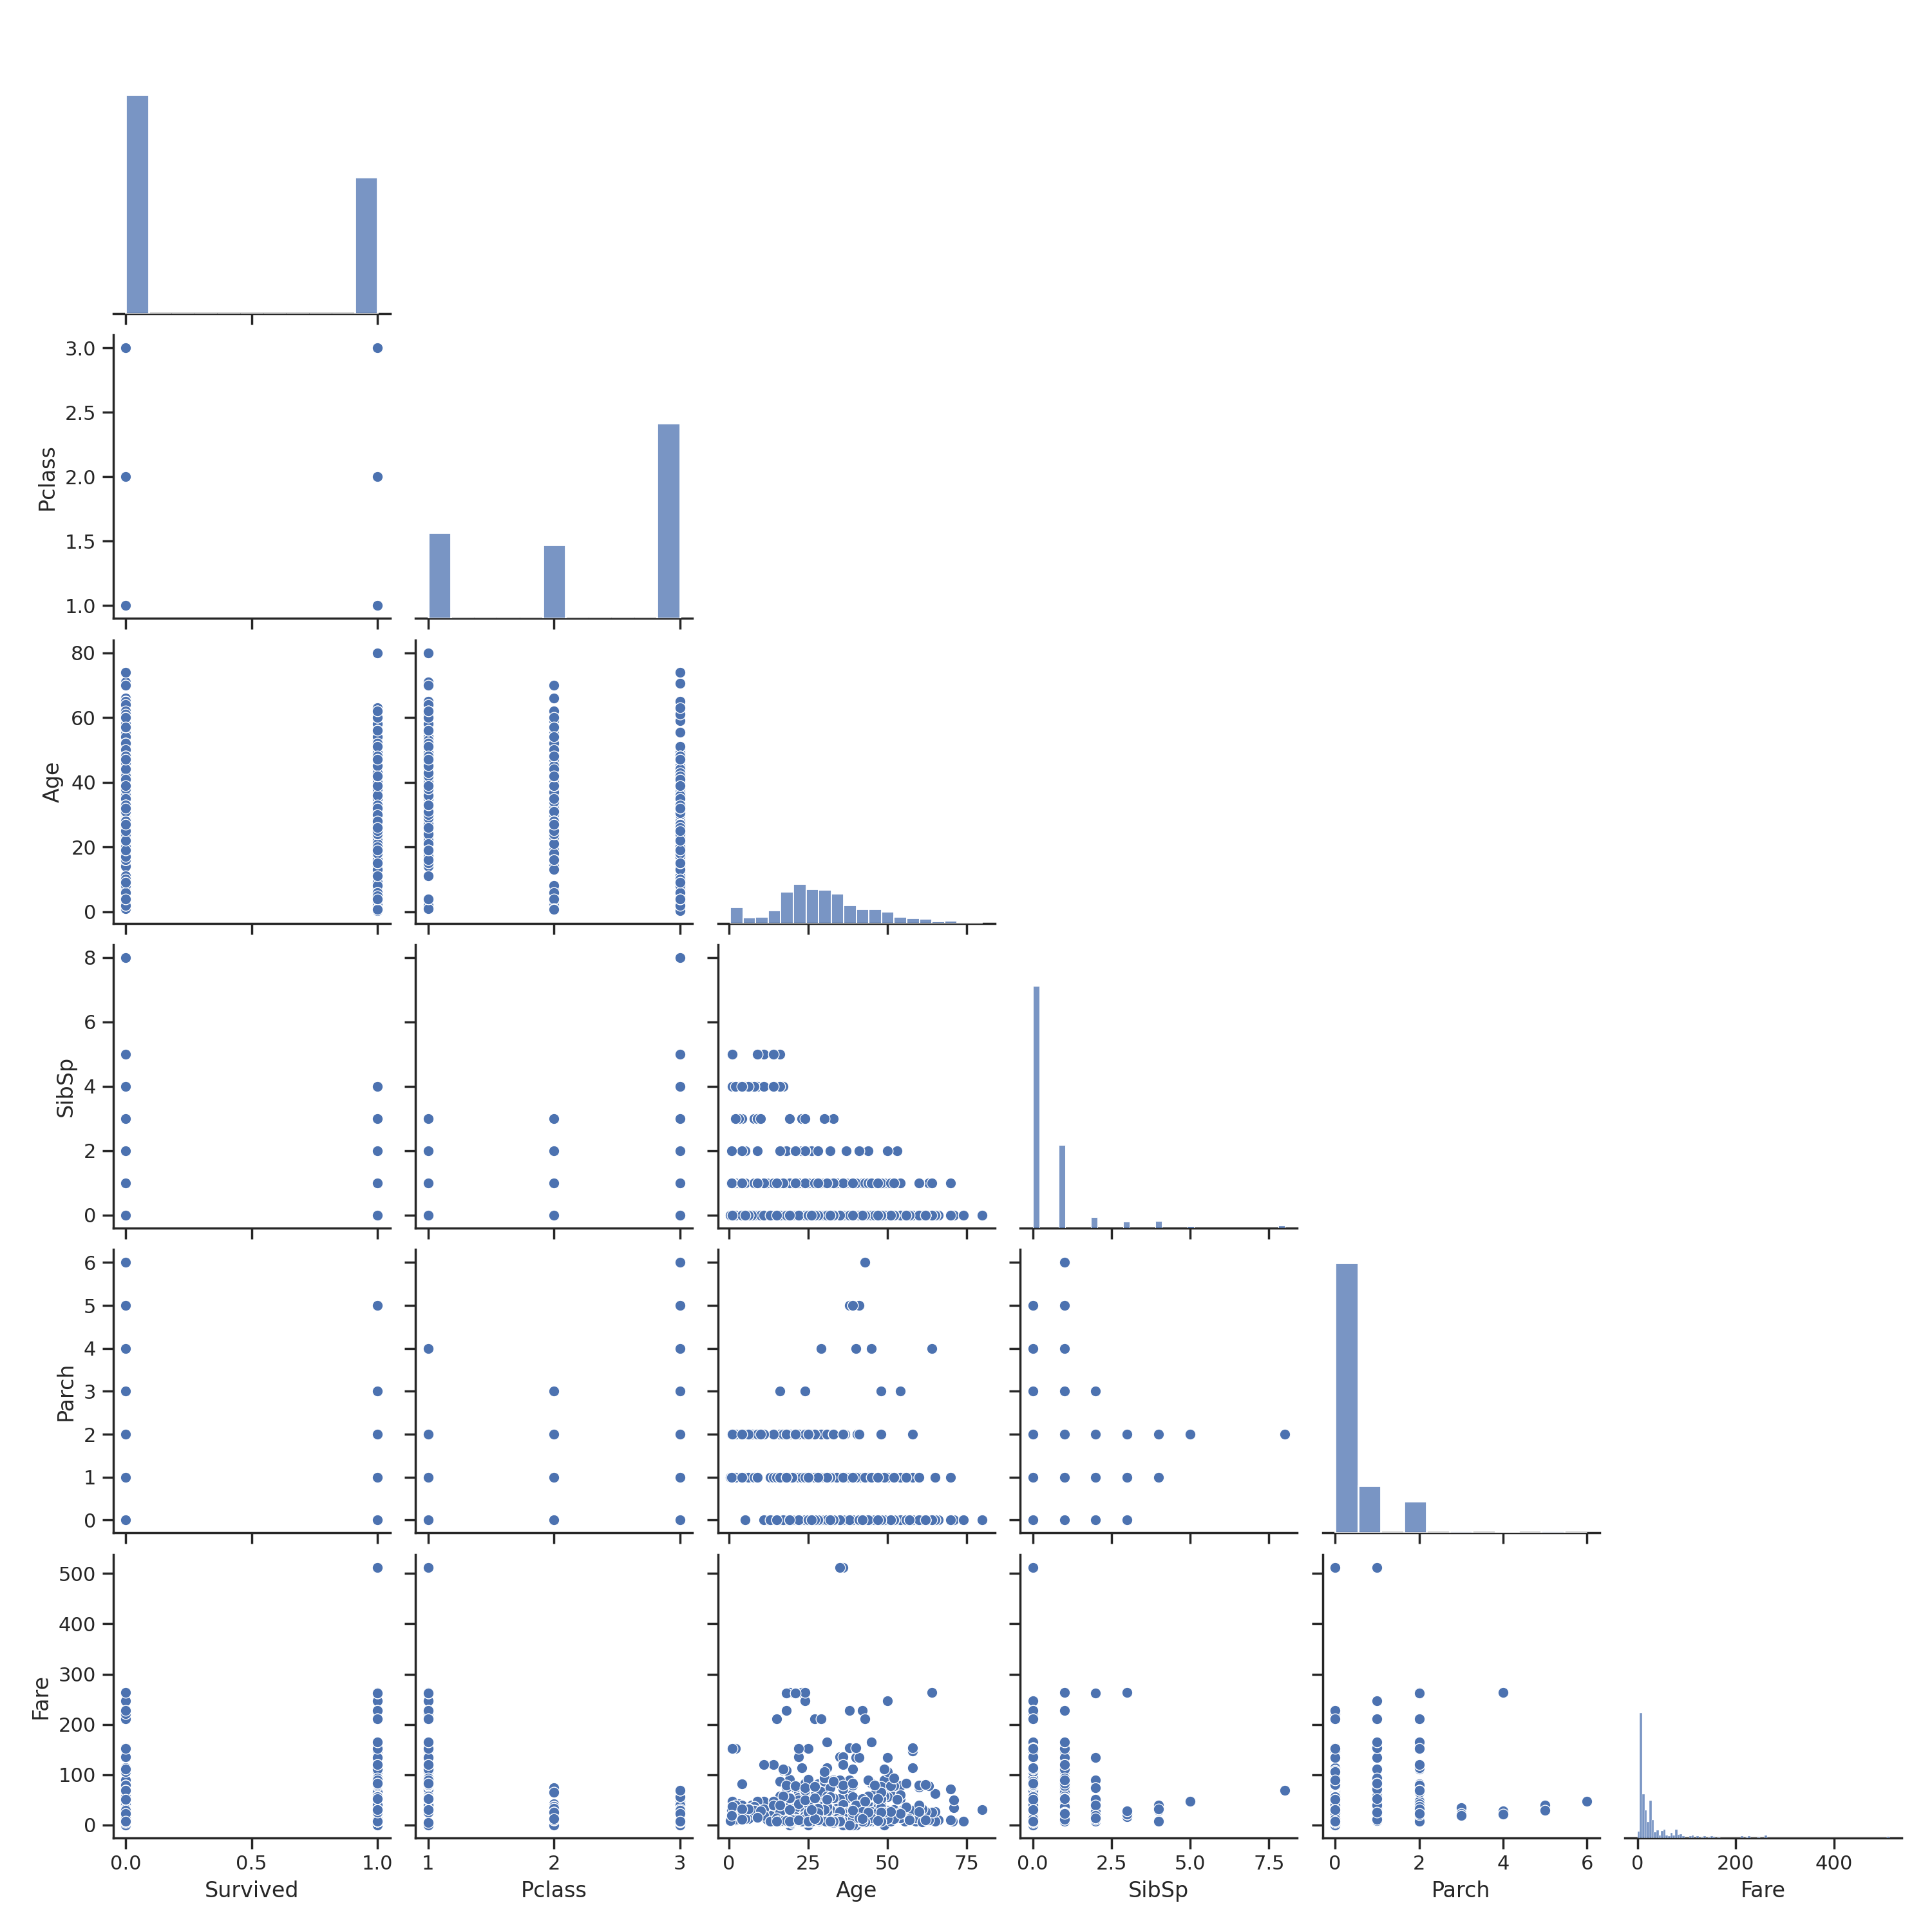
\includegraphics[width=\textwidth]{../plots/titanic_pairplot.png}
	\caption{ Distributions and pair-wise correlation for the features of the "Titanic" data set.}
	\label{pairplot_income}
\end{figure}


\begin{figure}[h!]
	\centering
	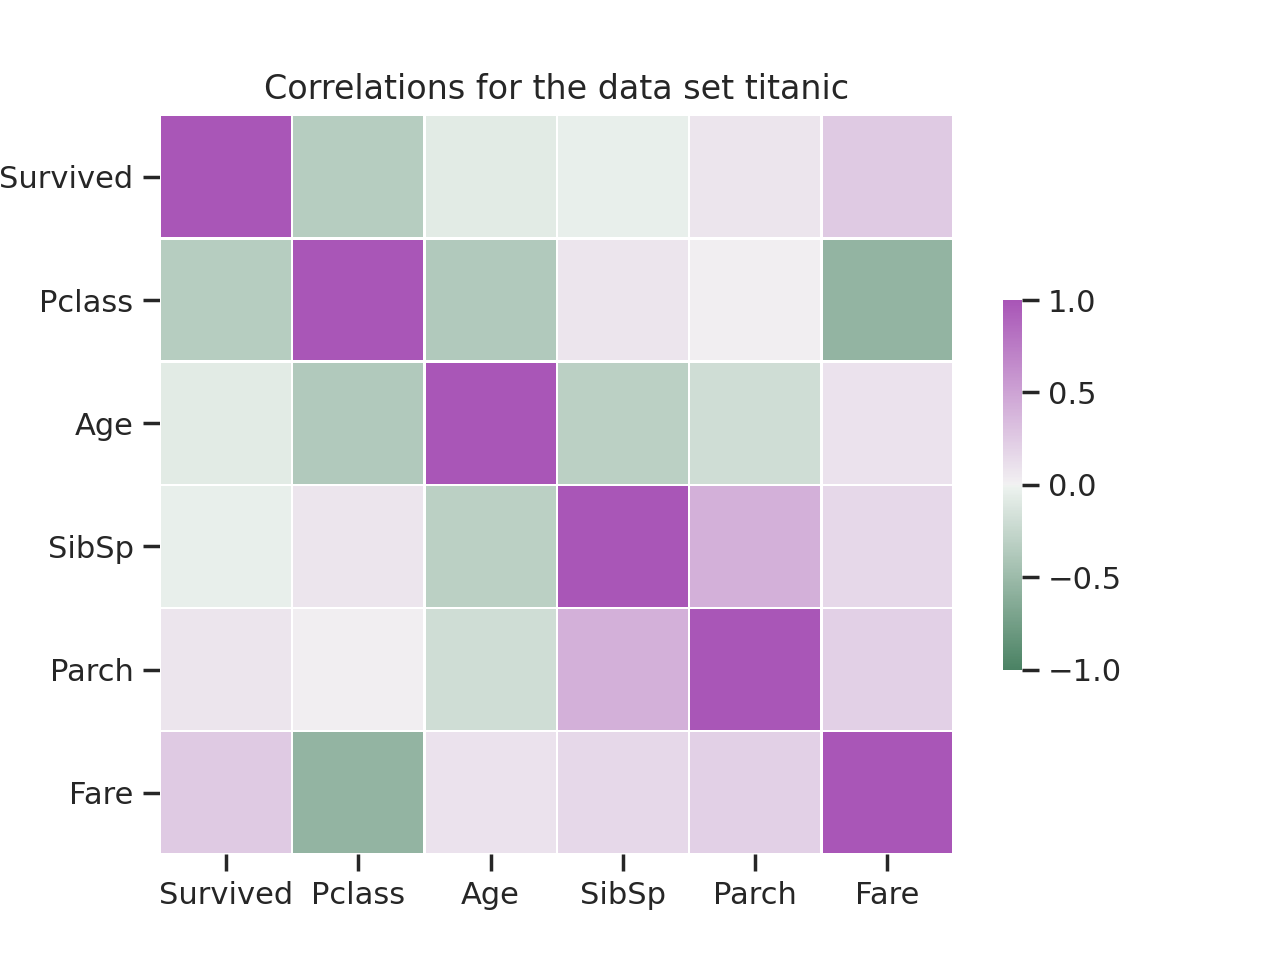
\includegraphics[width=0.7\textwidth]{../plots/titanic_correlations.png}
	\caption{Correlation matrix for the "Titanic" data set. }
	\label{correlation_income}
\end{figure}


\section{Workflow Overview and Code Structure}
Here we outline the structure of the code. The Project is build using the \textit{python3.8} language and various standard libraries such as \textit{pandas} and \textit{numpy} (for basic data import and analysis), \textit{sklearn} (sci-kit learn for model training and evaluation), \textit{} (for the creation of the synthetic data sets), \textit{matplotlib} and \textit{seaborn} for data visualization. 

The project includes five different scripts that perform different tasks:

\begin{itemize}
	\item \textit{clean\_dataset.py}: module for the loading and cleaning of the input data sets. It reads the input data sets ad \textit{pandas} data frames, which are the main format handled by the library for model training. Among the cleaning of the data, we find the outlier removals and data rescaling;\
	
	\item  \textit{generate\_data.py}: module for the creating of synthetic data, based on the \textit{SDV} library;\
	
	
	\item  \textit{classifier.py}: main module of the project, contains the main functionalities to perform all the steps from data loading, cleaning, generation of synthetic data, model training and comparison of results;\
	
	\item \textit{utils.py}: module containing utilities e.g. for data plotting;\
	 
\end{itemize}

To run the entire project it is sufficient to call the \textit{classifier.py} module e.g. 
\begin{verbatim} 
python3.8 classifier.py 
\end{verbatim} 


\section{Data Exploration and Pre-processing}
In this section we describe the necessary preliminary steps to import and prepare the data to make them suitable for the learning algorithms.

The steps are handled by the script \textit{data\_preparation.py} which includes dedicated function to pre-process each data set.

\subsection{Data Overview}
Here we provide an overview of the original data.

\paragraph{Missing Value}
The
\paragraph{Normalization}
The
\paragraph{Labelling}
In all datasets were present not numeric features. In order to synthetize them was necessary to change the strings into numeric values. In order to do so we used the cat.code method in this way for every not numeric features all the possible values where labelled using a different value. Using the labelling we had the possibility to use the three models.

\section{Generation of Synthetic Data}
In order to generate the synthetic data we relied on three different generation models. The models are defined in the \textit{SDV} library. The three models aim to generate a synthetic data set whose properties are the same as in the original dataset. The three models we used are: GaussianCopula model, CTGAN model, CopulaGAN model.
We now describe the idea behind these three models as reported on the SDV library user guide.

\paragraph{GaussianCopula}
The Gaussian copula model \cite{gaussiancopula} is based on copulas which are distributions on [0;1]$^d$ which is constructed from a multivariate normal distribution over $\mathbb{R}^d$ by using the probability integral transform. Intuitively, a copula is a mathematical function that allows us to describe the joint distribution of multiple random variables by analyzing the dependencies between their marginal distributions.
\paragraph{CTGAN model}
The sdv.tabular.CTGAN model \cite{ctgan} is based on the GAN-based Deep Learning data synthesizer which was presented at the NeurIPS 2020 conference by the paper titled "Modeling Tabular data using Conditional GAN".
\paragraph{Copula GAN}
The sdv.tabular.CopulaGAN model \cite{copulagan} is a variation of the CTGAN Model which takes advantage of the CDF based transformation that the GaussianCopulas apply to make the underlying CTGAN model task of learning the data easier.

\section{Model Implementation}

\subsection{Holdout and Cross Validation}
Here we describe briefly the techniques of "holdout" and "cross validation" that are used to evaluate a model. The \textbf{holdout} method is essentially based on the splitting on the input data set into two subset, one used for training the model, and one used for testing the model, for example in $80\%-20\%$ proportion, although there is not fix recipe for this split. Once the model is trained, the evaluation can be performed on the test data set, and this is therefore possible to check if the prediction of the model match the data. One big issue of this model is that the training strongly depend on the splitting of the initial data set, for example if the characteristic of the training data set are not representative of the whole data set.

A more powerful method is the \textbf{cross-validation} or "k-fold cross validation". Form the full dataset, a test is held out for final evaluation, but the validation set is no longer needed. For this, the training set is split into $k$ sets, so that the model is trained using $k-1$ folds as training data, and the remaining one is used for the validation as a test set (to compute the interesting metric of the model).
Once we obtain such $k$ number of metrics, the final result is the average of these parameters, obtained for each iteration of the cross-validation on each distinct fold.


\section{Performance Tests}

\paragraph{Confusion Matrix}
For each classifier, we produce a confusion matrix where each entry $i,j$ corresponds to the number of observations in group $i$, but predicted to be in group $j$. We chose to normalize the entries according to the sum of each row.
In case of binary classification, the matrix reduces to the number of true negatives ($TN$), false positives ($FP$), false negatives ($FN$) and true positives ($TP$).

Examples can be see in Fig. \ref{confusion_matrices}.

We remind here the definition of the metric parameters we will used to quantify the performance of our classifiers i.e. precision ($P$), recall ($R$) , accuracy ($A$) and specificity $S$:

\begin{equation}
P = \frac{TP}{TP + FP} \ \ \ \ \ \ \ \  R = \frac{TP}{TP + FN} \ \ \ \ \ \ \ \  A = \frac{TP + TN}{all}
\ \ \ \ \ \ \ \  S = \frac{TN}{TN + FP}
\end{equation}

It is straightforward to calculate these parameters for binary classification tasks out of the confusion matrix. In case of multiple labels, we need to calculate these parameter for each class, given that:
\begin{enumerate}
	\item  $TPs$ are the values in the diagonal; \
	\item  $FNs$ for a certain class are the sum of values in the corresponding row excluding the $TP$; \
	\item  $FPs$ for a certain class are the sum of values in the corresponding column excluding the $TP$; \
	\item  $TNs$ for a certain class are the sum of all rows and columns, excluding the class's column and row. \
\end{enumerate}


Another convenient metric, particularly because it is calculated directly from the proper \textit{scikit-learn} function, is called $f1-score$, which is defined as the harmonic mean of the precision and recall:
\begin{equation}
f1-score = 2 \times \frac{P \dot R }{P + R }
\end{equation}



\iffalse
\begin{figure}[h!]
	\centering
	\begin{minipage}[b]{0.49\textwidth}
		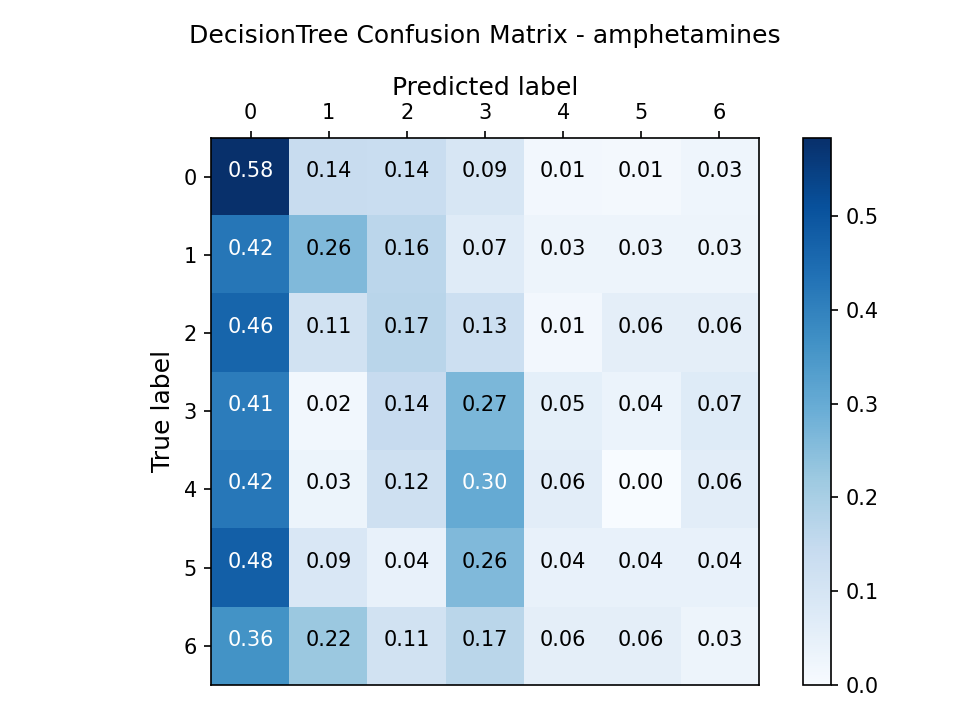
\includegraphics[width=\textwidth]{plots/m2.png}
	\end{minipage}
	\begin{minipage}[b]{0.49\textwidth}
		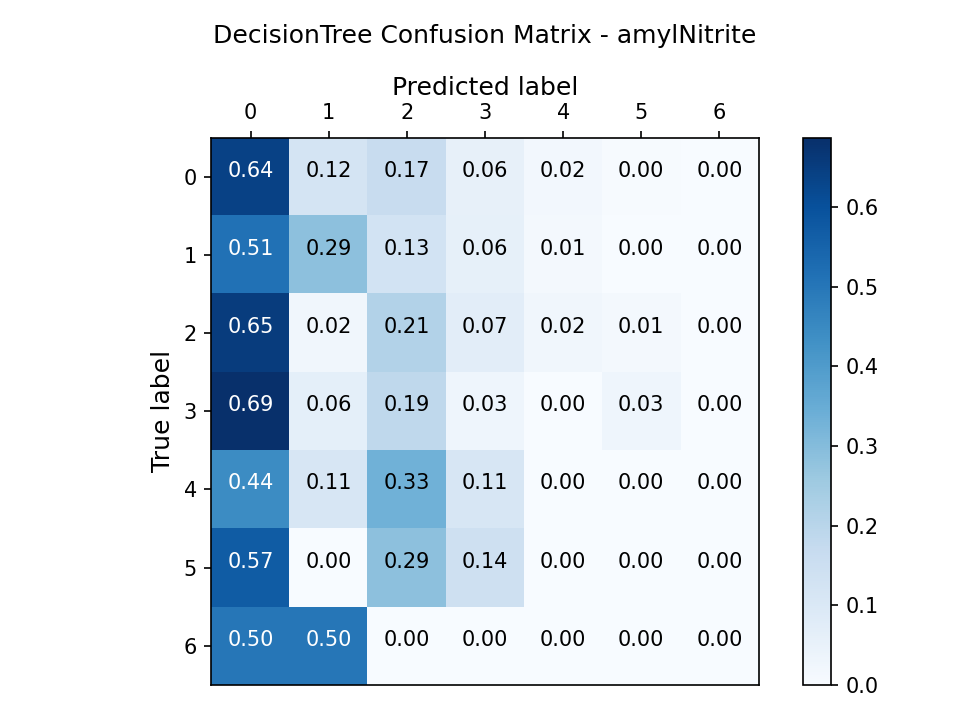
\includegraphics[width=\textwidth]{plots/m1.png}
	\end{minipage}
	\caption{Example confusion matrices for {\color{red} XXX }  }
	\label{confusion_matrices}
\end{figure}
\fi

{\color{red} Describe micro averaging and macro averaging, will we report both ? }

\section{Conclusion}

\clearpage
\bibliography{literature.bib}{}
\bibliographystyle{unsrt}

\end{document}
